% -------------------------------------------------------------------------------- %
% Latex file: `section-experiments.tex`
% Description:
% Use it to collect and show different slides about experiments carried out.
% -------------------------------------------------------------------------------- %

% Experiments
% -----------------------------
\section{Experiments}
    \subsection{Experiemnt Design Choices and Results}

        \subsubsection{Automated Gradual Pruning Technique}
        % -------------------------------------------------------------------------------- %
% Latex file: `agp-pruning-theory.tex`
% Description:
% Speaing about Automated Gradual Pruning Technique
% reporting in a summarized way its major properties and characteristics.
% -------------------------------------------------------------------------------- %

% Automated Gradual Pruner
% -------------------------------------------------------------------------------- %
\begin{frame}
    \frametitle{Automated Gradual Pruner}
        % \centering \Huge
        \begin{center}
            {\fontsize{40}{50}\selectfont \emph{Automated Gradual Pruner}}
        \end{center}
        \begin{center}
            \emph{Deep Neural Network Pruning Based Compression Techinque}
        \end{center}
\end{frame}

% AGP  Part n°1: Automated Gradual Pruner
% -------------------------------------------------------------------------------- %
\begin{frame}
    \frametitle{Automated Gradual Pruner}
        \textbf{Automated Gradual Pruner (AGP)}, discussed in \textbf{To prune, or not to prune: exploring the efficacy of pruning for model compression},
            the authors Michael Zhu and Suyog Gupta propose an intuitive, fresh new pruning approach briefly described as:

        \begin{itemize}
        \item \textbf{new automated gradual pruning algorithm} in which the sparsity is increased from an initial sparsity value $s_{i}$ (usually 0)
            to a final sparsity value $s_{f}$ over a span of $n$ pruning steps;
        \item The intuition behind this sparsity function in equation below is to \textbf{prune the network rapidly in the initial phase} when:
            \begin{itemize}
                \item the redundant connections are abundant, and;
                \item gradually reduce the number of weights being pruned each time as there are fewer and fewer weights remaining in the network.
            \end{itemize}
        \end{itemize}

    % \begin{equation}
    % s_{t} = s_{f} + (s_{i} - s_{f}(1 - \frac{t-t_{0}}{n \Delta t})^{3}), t \in \{t_{0}, t_{0} + \Delta t, \dots, t_{0} + \Delta n\}
    % \end{equation}
\end{frame}


% AGP  Part n°2: Automated Gradual Pruner (2)
% -------------------------------------------------------------------------------- %
\begin{frame}
    \frametitle{Automated Gradual Pruner (2)}
        Other interesting properties related to \textbf{Automated Gradual Pruner (AGP)}, and discussedwithin Michael Zhu and Suyog Gupta's paper,
            for better appreciating and understanding the usefulness of such a technique are:

        \begin{itemize}
        \item It Requires a lower number of trials, and attempts for identifying meaningful set of hyper-params for leading the pruning approach,
            compared to other techniques such Magnitude Level Pruning and other similars;
        \item It does not made particular assumptions on weight values density distribution;
        \item It is agnostic with respect to the particular Deep Neural Network Architecture chosen;
        \end{itemize}
\end{frame}

        



\begin{frame}
\frametitle{Identifyed Target Image for Training Siren Models (2)}
Differently from Siren paper's Camera Image, we decide to resize it, by cropping the full image down to 256x256 image about its center, leading to the following update image:


\begin{columns}
\column{0.5\textwidth}
\begin{figure}
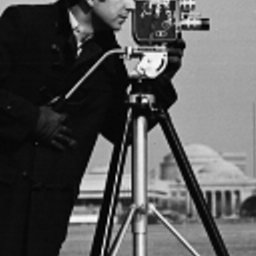
\includegraphics[scale=0.2]{slides/experiments/target-image/cropped_cameramen_256x256.png}
\caption{Camera 256x256 target image}
\end{figure}

\column{0.5\textwidth}
\begin{table}
\begin{tabular}{ll}
\hline
          Image Feature & Value \\
\hline
       name &      Camera \\
      shape &  (256, 256) \\
  size\_byte &       65536 \\
 image\_band &        (L,) \\
\hline
\end{tabular}
\caption{Cropped Camera Image Characteristics }
\end{table}

\end{columns}
\end{frame}

\begin{frame}
\frametitle{Data Distribution for Target Image for Training Siren Models}

\begin{figure}
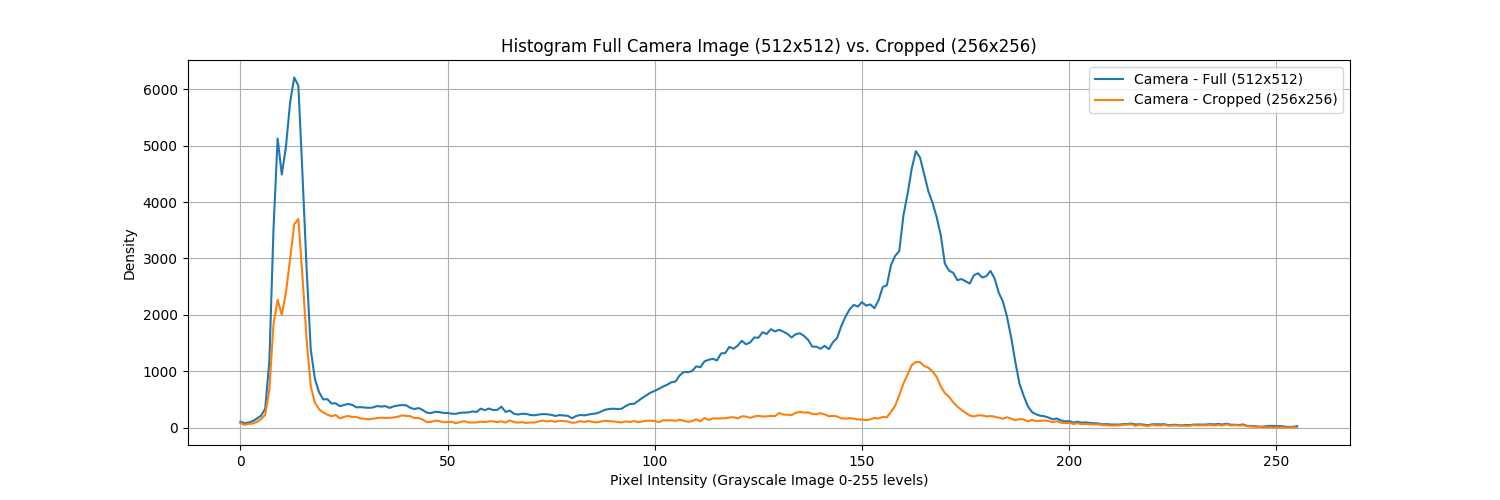
\includegraphics[scale=0.2]{slides/experiments/target-image/mixing_image_hist.png}
\caption{Camera target image, full and cropped data distribution}
\end{figure}

\end{frame}


\begin{frame}
\frametitle{General Summarizing Image Overview}
\begin{figure}
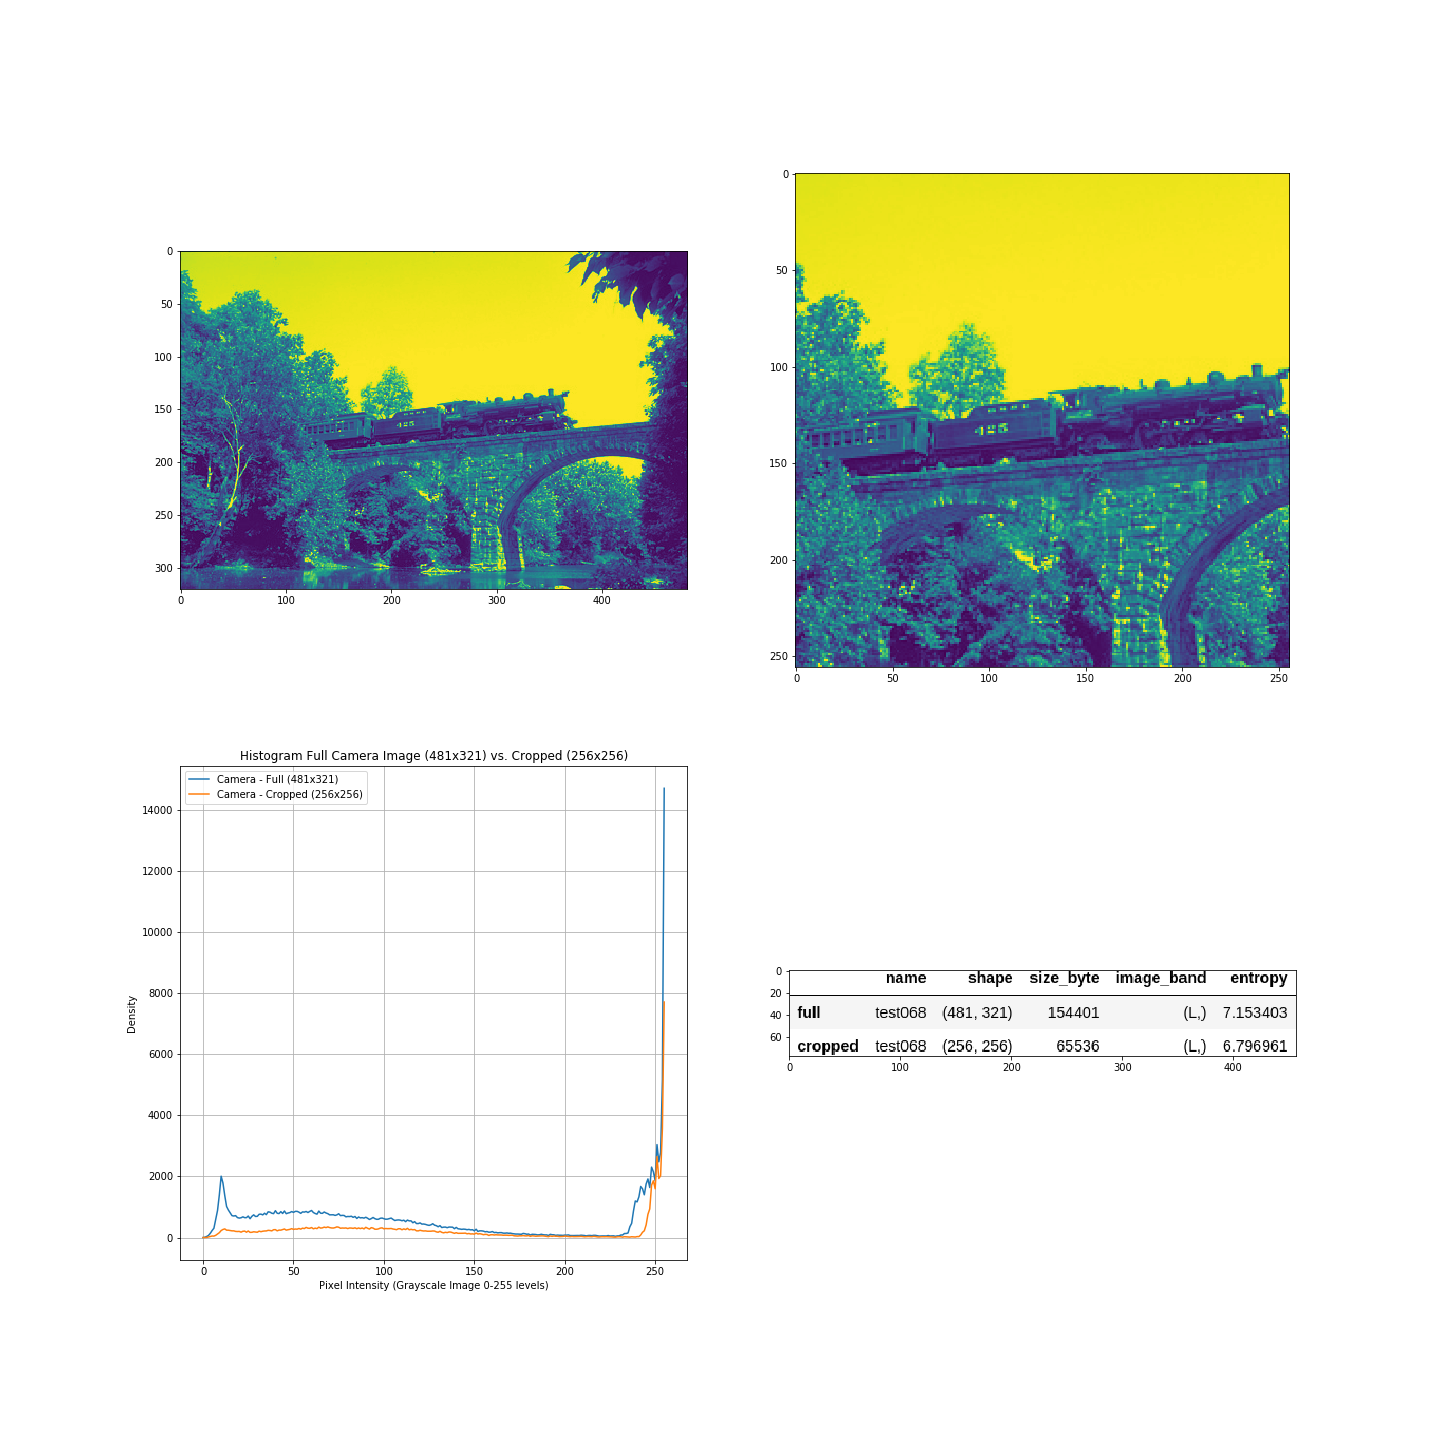
\includegraphics[scale=0.15]{slides/experiments/target-image/complex_3.png}
\end{figure}
\end{frame}
        % -------------------------------------------------------------------------------- %
% Latex file: `control-group-image.tex`
% Description:
% Speaking about cropped image cameramen Jpeg and Plain Siren Trained 
% Models, picture details.
% -------------------------------------------------------------------------------- %

% Pnsr [db] vs. Bpp for Jpeg Compressed Image and Siren Trained Models
% -------------------------------------------------------------------------------- %
\begin{frame}
    \frametitle{Base Pnsr [db] vs. Bpp Jpeg Scatterplot}
    \begin{figure}
    % 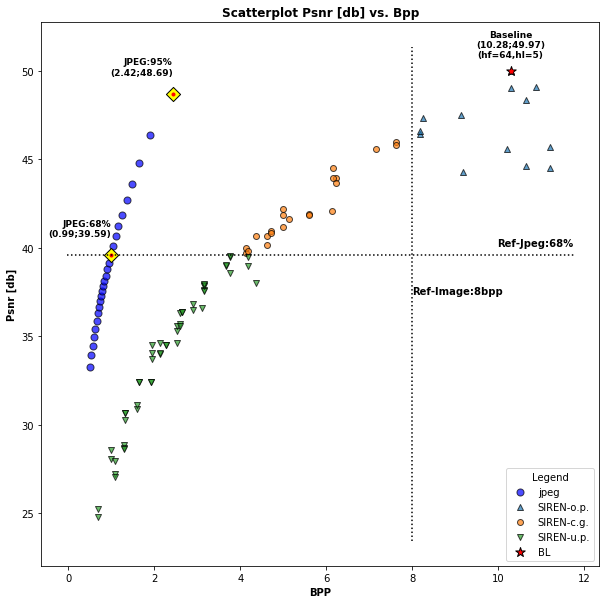
\includegraphics[scale=0.35]{slides/experiments/target-image/images/tmp_scatterplot_quant.png}
    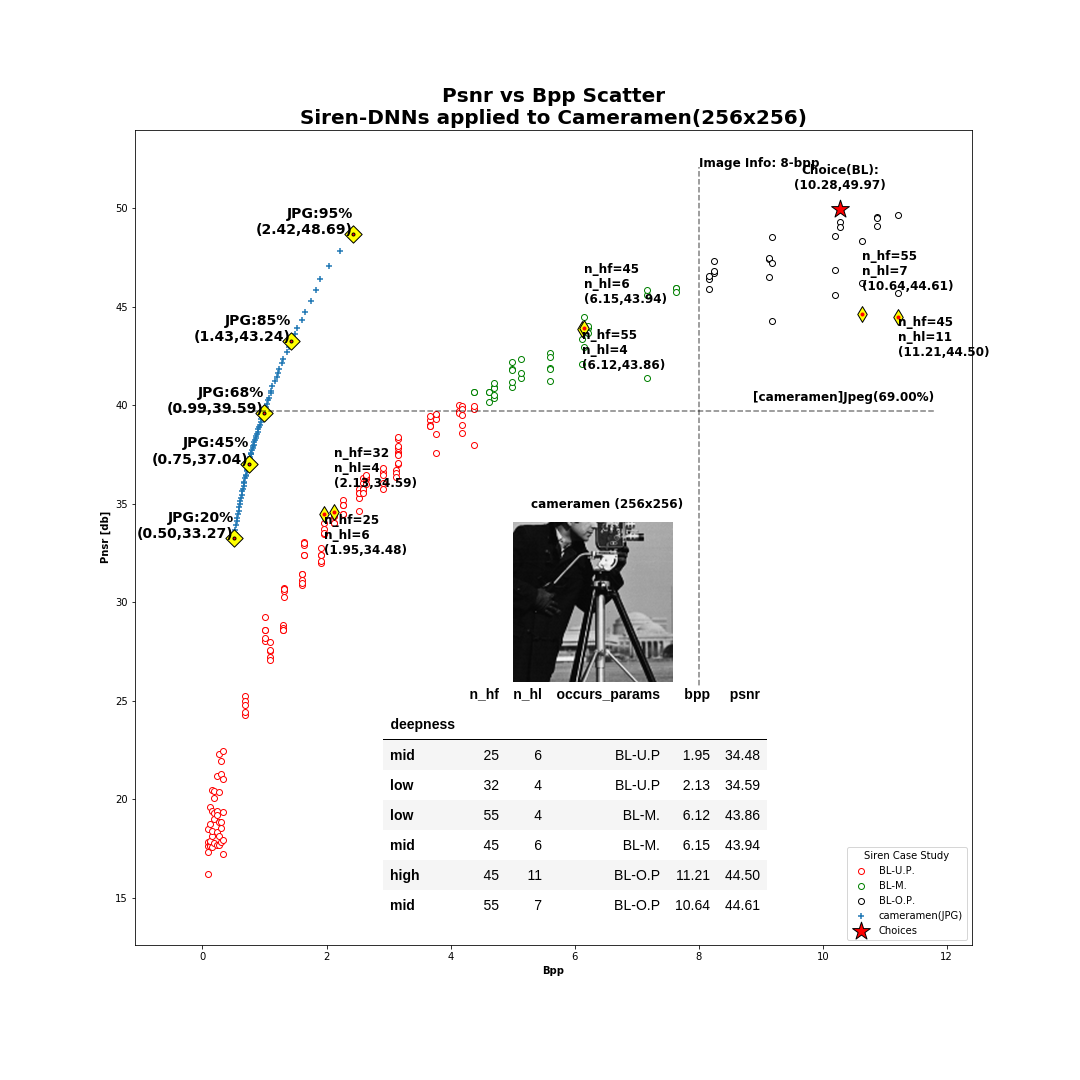
\includegraphics[scale=0.23]{slides/experiments/target-image/images/cameramen_jpeg_plain_siren_1.png}
    \caption{Jpeg, Plain Siren Architecture Control Groups}
    \end{figure}
\end{frame}

        



\begin{frame}
\frametitle{Pruning Technique Workflow}
For pruning Siren based Deep Models via AGP pruning method, and after having performed some random trials, via \textbf{Random Search Approach} to indetify most suitable hyper-params, we follow the subsequent training strategy:
\begin{itemize}
\item We determine the degree of pruning for each layer depending on the \textbf{Sensitivity Level Analysis} done ahead of pruning time.
\item We let the \textbf{Frequency} Hyper-parameter to be picked up from: $\{50, 100, 200\}$ possible choices, essential to let net model to mitigate or recovery from \textbf{brain damage} induced while removing not salient weigths;
\item We train each model for a \textbf{Number of Epochs} equals to $150000$ before turning off pruning and let the model to finish remaining epochs;
\item We both train \textbf{from scratch} by means of AGP algorithm or prune an \textbf{already trained, for reaching overfitting state, models};
\item We follow a generically \textbf{Suggested Heuristic in literature} for not pruning first and last layers in order to let performance to not degradate too much;
\end{itemize}

\end{frame}

        



\begin{frame}
\frametitle{AGP Pruning Technique: obtained results}

\begin{figure}
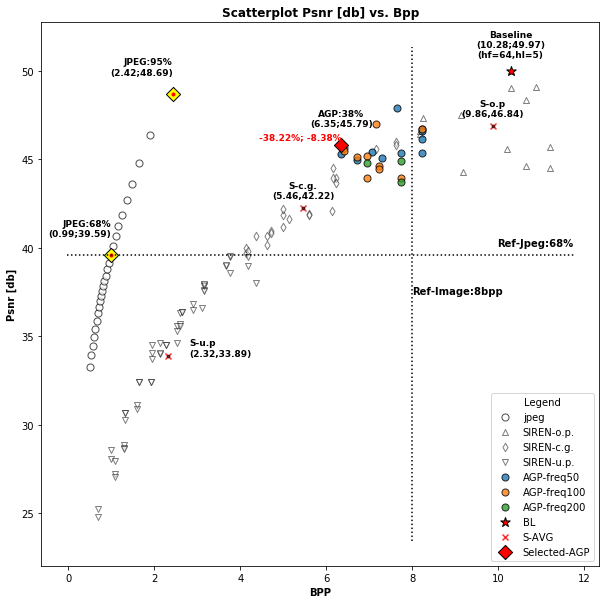
\includegraphics[scale=0.40]{slides/experiments/pruning-tech/tmp_scatterplot_pruning.png}
\end{figure}

\end{frame}


        \subsubsection{Linear Range Quantization Technique}
        



% -------------------------------------------------------------------------------- %
\begin{frame}
    \frametitle{Selected Deep Nets Compression Techniques}
        % \centering \Huge
        \begin{center}
            {\fontsize{40}{50}\selectfont \emph{Range Linear Quantization}}
        \end{center}
        \begin{center}
            \emph{Quantization Aware Training Technique for Compressing Deep Nets}
        \end{center}
\end{frame}


% -------------------------------------------------------------------------------- %
\begin{frame}
    \frametitle{Linear Range Quant}
        In order to satisfy quantizing requirements we made use of Linear Range Quantization technique, which is a Quant Aware Training method developed by
        Benoit et al, (2018), whose main features are:

        \begin{itemize}
            \item \textbf{quantization scheme} that relies only on integer arithmetic to approximate the floating-point computations in a neural network;
            \item \textbf{Training Procedure} that simulates the effect of quantization helps to restore model accuracy to near-identical
                levels as the original.
            \item The Algorithm uses exponential moving averages to track activation ranges.
        \end{itemize}
\end{frame}


% -------------------------------------------------------------------------------- %
\begin{frame}
    \frametitle{Linear Range Quant (2)}
        In order to satisfy quantizing requirements we made use of Linear Range Quantization technique, which is a Quant Aware Training method developed by
        Benoit et al, (2018), whose main features are:

        \begin{itemize}
        \item They requiring that thequantization scheme be anaffine mapping of integers $q$ toreal numbers $r$, i.e. of the form:
        \begin{equation}
            r = S(q - Z)
        \end{equation}
        for some constants S and Z quant-parameters.
        \item where, The constant S (for “scale”) is an arbitrary positive realnumber. It is typically represented in software as a floating-point quantity,
            like the real values $r$.
        \item The constant Z (for “zero-point”) is of the same type as quantized values $q$, and is in fact the quantized value $q$ corresponding
            to the real value 0.
        \item Finally, The motivationfor this requirement is that efficient implementation of neural network operators
            often requires zero-padding of arraysaround boundaries.

        \end{itemize}
\end{frame}

        



\begin{frame}
\frametitle{Linear Range Quant Workflow}
For pruning Siren based Deep Models via AGP pruning method, and after having performed some random trials, via \textbf{Random Search Approach} to indetify most suitable hyper-params, we follow the subsequent training strategy:
\begin{itemize}
\item We determine the degree of pruning for each layer depending on the \textbf{Sensitivity Level Analysis} done ahead of pruning time.
\item We let the \textbf{Frequency} Hyper-parameter to be picked up from: $\{50, 100, 200\}$ possible choices, essential to let net model to mitigate or recovery from \textbf{brain damage} induced while removing not salient weigths;
\item We train each model for a \textbf{Number of Epochs} equals to $150000$ before turning off pruning and let the model to finish remaining epochs;
\item We both train \textbf{from scratch} by means of AGP algorithm or prune an \textbf{already trained, for reaching overfitting state, models};
\item We follow a generically \textbf{Suggested Heuristic in literature} for not pruning first and last layers in order to let performance to not degradate too much;
\end{itemize}

\end{frame}

        



\begin{frame}
\frametitle{Linear Range Quantization: obtained results}

\begin{figure}
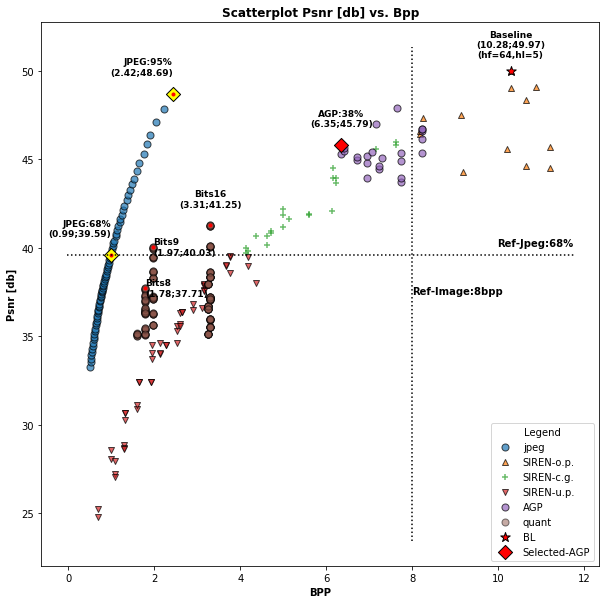
\includegraphics[scale=0.40]{slides/experiments/quant_dataset/tmp_scatterplot_quant.png}
\end{figure}

\end{frame}

